% This thesis is built on the belief that ...
% This chapter evaluates the  ...

Our aim is to validate our analysis about the trade-offs resulting from placing query processing state close to the clients
versus close to the database,
and to evaluate

% The following experiments aim to answer the following questions:

% Q ()

\section{Experimental scenario}

The evaluation in this chapter in the context of the case study presented in Section~\ref{sec:lobsters},
which describes the Lobsters \cite{lobste:rs} web application.
We have chosen this application because it is characterized by a read-heavy workload that requires the materialization
of derived state.
Moreover, the derived state is updated by a stream of small updates.
These characteristics make Lobsters suitable for evaluates the efficacy of our design and prototype implementation in
navigating the trade-offs of query processing state placement.
In addition, the Lobsters application is open-source \cite{lobsters:source},
allowing us to examine the application's interaction with the database,
and statistics about the applications data distributions and access patterns are available \cite{lobste:stats}.
Finally, Lobsters resembles a class of popular large-scale applications, such as Reddit and Hacker News.

\bigskip
\noindent
In Lobsters, users post, comment, and vote on ``stories''.
Each story is associated with a ``hotness'' value that indicates how popular it is
Stories are ranked based on their hotness;
the highest ranked stories appear on the front page.
The hotness value of a story depends on parameters such as the number of votes a story has gotten,
the number of comments, and the hotness of those comments.
As a result, various operations, such as voting or comment on a story, modify its hotness value.
It is prohibitively expensive \cite{gjengset:noria} to compute to hotness value of stories during queries.
In particular, serving Lobsters' front page requires computing the hotness of every story in order to rank them.
That is why the Lobsters application instead adds an additional column to the $stories$ table (the Lobsters application
uses MySQL for storing its state) storing the computed hotness value for each story.
The application updates the value of the hotness column when operations such as upvoting or downvoting a story, or
adding a comment to a story are performed.

For this evaluation, we consider a simplified version of the Lobsters application.
In particular, we consider the following database schema:

\begin{lstlisting}[
          language=SQL,
          showspaces=false,
          basicstyle=\ttfamily,
          commentstyle=\color{gray},
          rulecolor=\color{black},
          stringstyle=\color{mymauve},
          frame=L,
          xleftmargin=\parindent,
          commentstyle = \color{gray}
        ]
TABLE users (id bigint, username varchar(50))
TABLE stories (id bigint, user_id bigint, title varchar(150), description mediumtext, short_id varchar(6));
TABLE votes (id bigint, user_id bigint, story_id bigint, vote tinyint);
\end{lstlisting}

In addition, we consider a workload consisting for two operations: voting up or down a given story and requesting the Lobsters
front page.
The front page is a listing of the 25 most highly ranked stories, including their title, author, and vote count.
In the statistics provided by the Lobsters administrators, the front page operation constitutes 30.1\% of client requests,
and voting on stories constitutes 0.5\% of client requests.
Our simplified workload consists of 95\% front page operations, and 5\% voting operations, unless otherwise specified.
We believe that this accurately represent the ration of read and write operations in the available Lobsters applications
statistics.

The evaluation uses the QPU architecture depicted in Figure~\ref{fig:eval_lobsters_qpu_arch}.
This architecture maintains a materialized view that integrates both integrates stories from the $stories$ table,
with their vote count.
The view definition the following query:

\begin{lstlisting}[
          language=SQL,
          showspaces=false,
          basicstyle=\ttfamily,
          commentstyle=\color{gray},
          rulecolor=\color{black},
          stringstyle=\color{mymauve},
          frame=L,
          xleftmargin=\parindent,
          commentstyle = \color{gray}
        ]
SELECT id, author_id, title, url, vote_count
FROM stories
JOIN (
  SELECT story_id, SUM(vote) as vote_count
  FROM votes
  GROUP BY story_id
) view
ON stories.id = view.story_id
\end{lstlisting}

This simplifies both the vote and front page operation:
the vote operation does not need to explicitly update the hotness (here the vote count) of the given story as this
is performed by the QPU graph,
and the front page operation can be served from the materialized view.
We use an index on the materialized view to support efficient retrieval of the stories with the highest vote count.

\bigskip
\noindent
We consider a system architecture consisting of two geographically distant sites:
The Lobsters application is deployed on one site (we henceforth refer to this site as application site),
and clients are located on another site (client site).
Round-trip time between these two sites is 80ms.
We have chosen this value because it the the round trip time we observed between server in two OVH data centers,
one in Europe, and one in North America.
This value is relatively close to the round-trip times on AWS EC2, presented in \cite{pbailis:hats} (108ms between Ireland and N. Virginia).
This system model corresponds to a scenario in which a web application serves clients located in geographically distant regions.

In our experiments, we employ the flexible placement of the QPU graph,
and deploy the root of the QPU graph in either in the application or the client site.
By comparing these to placement schemes, one in which the materialized view is placed close to the corpus and one in which
it is placed close to the clients, we aim is to validate our analysis about the trade-offs resulting from placement decisions,
and to evaluate the effectiveness of Proteus in navigating these trade-offs.

\section{Experimental Setup}

\todo{fix GET/stories/X}
\begin{figure}[t]
  \centering
    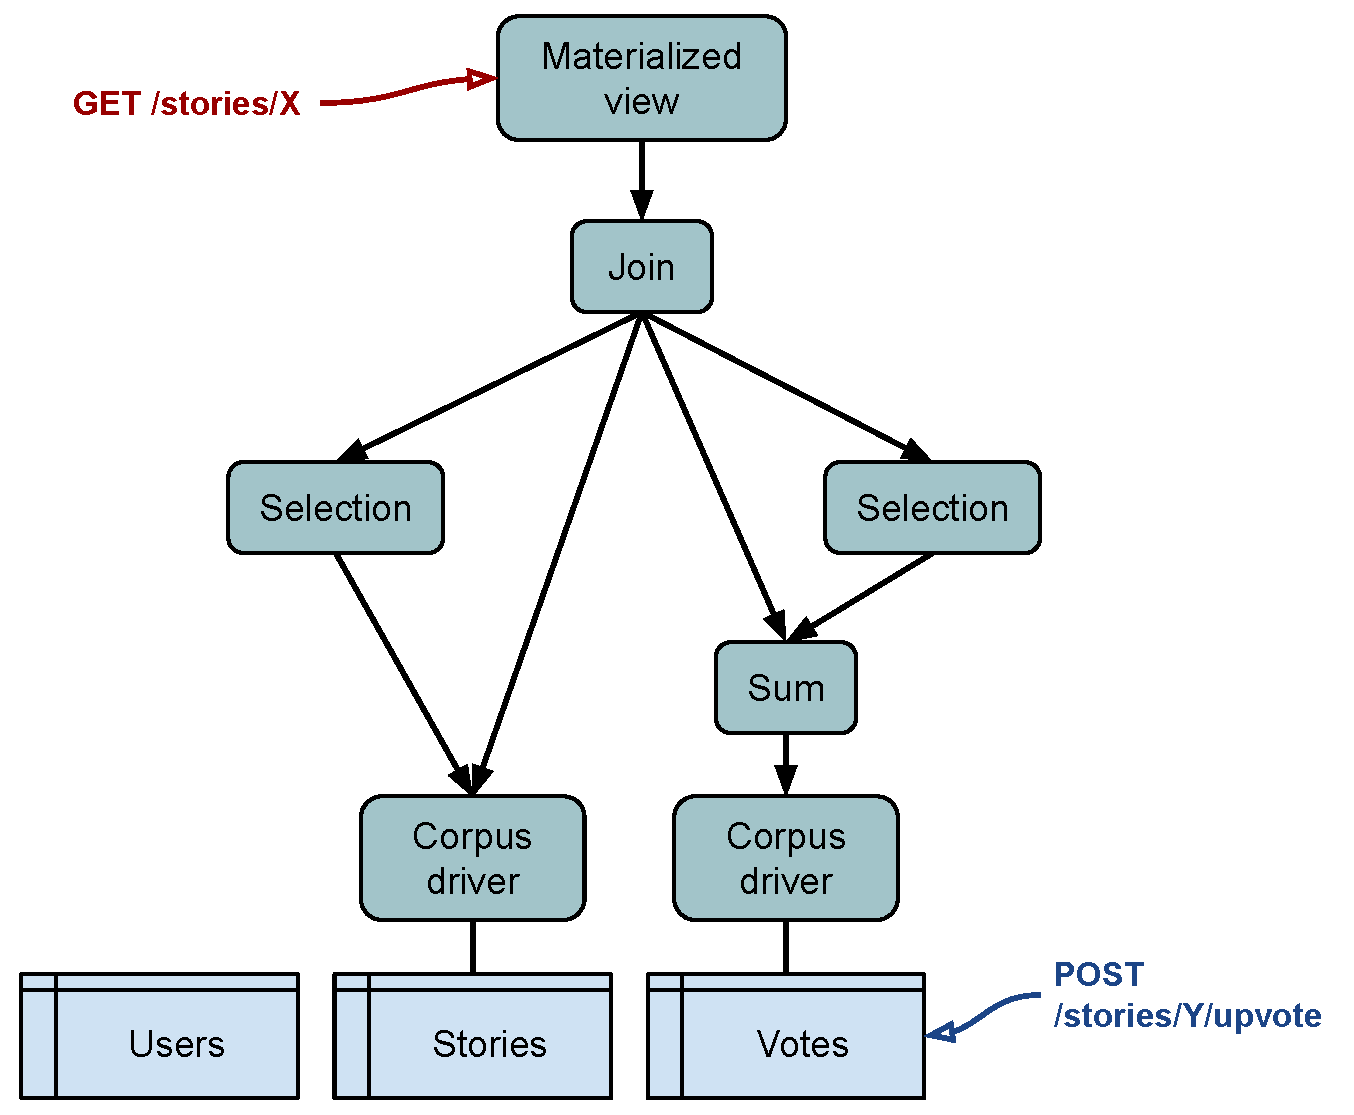
\includegraphics[scale=0.5]{./figures/case_studies/lobsters_architecture_basic.pdf}
  \caption{QPU architecture used for this evaluation. The materialized view QPU integrates stories with vote counts.
  The GET / request indicates the front page operation, and the POST /stories/Y/upvote request indicates the operation of voting up for story Y.}
  \label{fig:eval_lobsters_qpu_arch}
\end{figure}

This evaluation does not run the real Lobsters Ruby-on-Rails application.
Instead, we have implemented a adapter that translates user requests to queries that the real
Lobsters application would issue to the database,
and issues those queries either to MySQL, or MySQL and Proteus depending on the experiment configuration.
This allows us to isolate the interaction between Lobsters and the database, which is the focus of this work,
and remove other tasks of the Lobsters application that quickly become a bottleneck (such as rendering the frontpage).
This is a server-side adapter: it is deployed along with the database on the application site,
and plays the role of a web server.
The adapter exposes a gRPC endpoint, similar to the QPU gRPC server; clients issue operations as RPC requests.

\bigskip
\noindent
\textbf{Workload generation.}
For this evaluation, we have implemented a workload generator \cite{lobsters:bench} that is responsible for issuing
requests to the Lobsters adapter.
In addition, the workload generator measures request throughput and operation response time.
We define response time as the delay the client application experiences between issuing a request and receiving the
corresponding response.
To capture the variance of response time, we use a histogram data structure provided by the Go implementation of gRPC \cite{grpcgo:histogram}
that accumulates values in a histogram with exponentially increasing bucket sizes, and enables us to compute response time percentiles.

The workload generator uses an open-loop model \cite{schroeder:cautionarytale}:
the generator creates requests based on a target load value;
each request is executed by a separate thread (creating and destroying threads are low-cost operations because threads are
implemented as Goroutines).
The overall number of requests (and thus threads) that can be outstanding at a given point in time is bounded by a
configuration parameter.
When the bound is reached, additional requests need to wait for outstanding requests to be completed.
Our experiments showed that without the concurrency bound mechanism, when a threshold of outstanding gRPC requests is reached,
the server is overloaded and request latency increases by two orders of magnitude.

\bigskip
\noindent
\textbf{Freshness.} The materialized view provided by the QPU architecture is eventually consistent with the database state.
As a result, queries served from Proteus might provide reflect state that is stale relative to the database state.
In order to evaluate how stale query results are, we measure the freshness of the results of the front page operation.
We use two freshness metrics:
\begin{itemize}
  \item Update latency: the delay between a vote being committed in the database, and the updated vote count being committed
  in the materialized view.
  \item Returned version: How stale the returned version of a story is, measured as the number of versions to the version
  would have been read if reading from the database instead of Proteus.
\end{itemize}

We use the following mechanism to collect these two metrics.
For each vote operation, the MySQL logs the timestamp at which the corresponding transaction is committed;
this timestamp is then propagated to the QPU graph as an attribute, and stored by the materialized view in an
``update log'' table.
Additionally, the materialized view QPU logs the timestamp at the start of each query (building a ``query log'')
and the commit timestamp of each view update.
At the end of a benchmark run, the materialized view QPU performs a post mortem analysis:
The update latency is computed by subtracting the view update commit timestamp from the database transaction commit
timestamp.
The returned version for each frontpage story is computed by replaying the update history and determining and determining
how stale (measured in number of versions) was a story record in the materialized view compared to that story record in the database
when a given query was executed.

For freshness measurements benchmarks,
we deploy all system components (MySQL instance, QPU graph, and workload generator) on the same server in order to ensure
that timestamps in the database and materialized view QOU have the same source (Docker containers run on a Linux host use
the host system's clock).
This avoid issues caused by clock drift between servers.

\bigskip
\noindent
\textbf{Hardware.}
Experiments were run on a cluster located in Paris, provided by the Laboratoire d'Informatique de Paris 6 (LIP6).
Each server consists of 2 Intel Xeon E5645 CPUs, each with 6 cores, 64 GB RAM, an 128 GB SSD disk, and a 4 TB HDD disk.

\bigskip
\noindent
\textbf{Configuration.}
We simulate the two geographically distant sites using the Linux tc utility \cite{tc} to add delay to outgoing packets.
For response time measurements the MySQL instance and the QPU graph except the materialized view QPU are deployed on a single
server, while the join QPU and workload generator are deployed on separate, dedicated servers.

As described above, for the freshness measurements, all components are deployed on a single server.

Experiments run for 5 minutes unless otherwise specified, and staring taking measurements after an initial ``warmup period''
of 30 seconds.
Repeated run have shown that results are stable and consistent across multiple runs.

% \section{Navigating the design space of geo-distributed query}
% (Note: The title might be a bit too fancy. To re-think.)

% Question to answer:
% Can the QPU approach be used to adjust to navigate the design space
% geo-distributed query, making different trade-offs depending on the requirements
% and characteristics of specific applications.

% Hypothesis to validate:
% For a given pair of workload type (eg. query-heavy) and requirement (expressed
% as performance/efficiency metric) there is a query engine configuration that
% ''optimizes'' the given metric.

% (Idea on how to visualize this: 2D matrix ''workloads - metrics'':
% for each cell, find which configuration is best for this workload and metric.

% High-level plan:
% \begin{itemize}
%   \item Run a set of different workloads, measuring different metrics (query
%   performance, freshness, cost)
%   \item Repeat this for a set of query system configurations.
%   \item Examine for each worload-metric pair, how changing the query engine
%   configuration affects the target metric.
% \end{itemize}

% \section{Application benchmark}
% (Note: I ran out of inspiration for titles)

% Question to answer:
% What performance gains can the QPU approach deliver to an application, and how
% it Proteus compare against state-of-the-art systems?

% Hypotheses to validate
% \begin{itemize}
%   \item 1. The QPU approach (Proteus) can provide the performance comparable to
%   that of state-of-the-art systems when used with a similar configuration.
%   \item 2. The QPU approach (Proteus) can improve the application's performance
%   (or improve freshness or cut cost) by enabling query engine designs (placement
%   schemes, ...) not possible with current query systems.
% \end{itemize}

% (This is currently being designed and implemented.)